\usetikzlibrary{arrows.meta,calc}
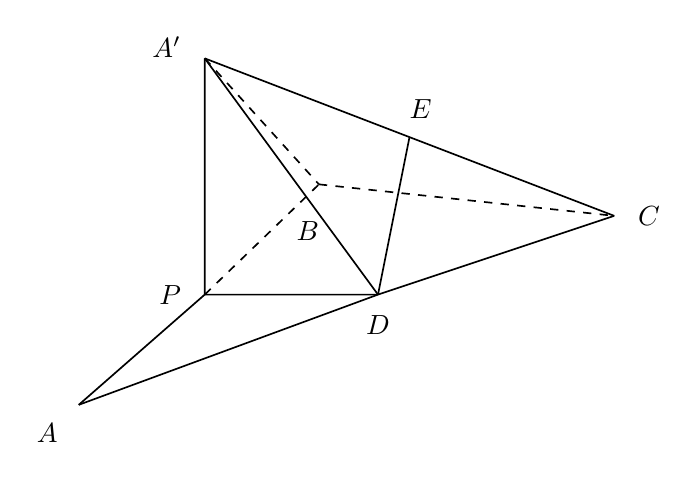
\begin{tikzpicture}[x=1cm,y=1cm,font=\normalsize,line width=.6pt]
\coordinate (Apr) at (0,4.2);
\coordinate (P) at (0,1.2);
\coordinate (B) at (1.4500000000,2.6000000000);
\coordinate (D) at (2.2,1.2);
\coordinate (C) at (5.2,2.2);
\coordinate (E) at (2.6000000000,3.2000000000);
\coordinate (A) at (-1.6,-0.2);
% solid outline
\draw[solid] (Apr)--(P)--(D)--(C);
\draw[solid] (Apr)--(D);
\draw[solid] (Apr) -- (C);

\draw[solid] (E) -- (D);
\draw[solid] (A) -- (P);
\draw[solid] (A) -- (D);
% dashed hidden
\draw[dashed] (Apr) -- (B);
\draw[dashed] (P) -- (B);
\draw[dashed] (B) -- (C);
% labels with clearance
\node[left,xshift=-5pt,yshift=4pt] at (Apr) {$A'$};
\node[left,xshift=-5pt] at (P) {$P$};
\node[below,xshift=-4pt,yshift=-10pt] at (B) {$B$};
\node[below,yshift=-4pt] at (D) {$D$};
\node[right,xshift=5pt] at (C) {$C$};
\node[above,xshift=4pt,yshift=3pt] at (E) {$E$};
\node[below left,xshift=-4pt,yshift=-3pt] at (A) {$A$};
\end{tikzpicture}
